\documentclass[]{article}
\newcommand{\FileDepth}{../../..}
\usepackage[letterpaper, landscape, margin=0.5cm]{geometry}
\usepackage[T1]{fontenc}
\usepackage{textcomp}%Not strictly necessary, but gives \textmu command for "micro."
\usepackage{fancyhdr}
\usepackage{amsmath}
\usepackage{amssymb}
\usepackage{graphicx}
\usepackage{xcolor}
\usepackage{tikz}
\usetikzlibrary{calc}
\usepackage{censor}
\usepackage{hyperref}
\usepackage{multicol}
%opening
\newcommand{\SecType}{L}
\newcommand{\Week}{2}
\title{PH 211 Lecture \Week}
\author{Benjamin Bauml}
\date{Summer 2024}

\newcommand{\Purpose}{4}
\newcommand{\DefOnly}{0}

\input{\FileDepth/Formats/Assignment20240614.tex}
\usepackage[absolute]{textpos}
% This package relies on Assignment Format 2024-06-14 or later to work. It is recommended that the Purpose and DefOnly commands be given as such:
%\newcommand{\Purpose}{4}
%\newcommand{\DefOnly}{0}
% Activities need to be entered outside of the TeacherMargin and PresentSpace environments, otherwise they will be defined only locally. They can even go in the preamble.
\newenvironment{TeacherMargin}{\begin{textblock*}{10.8cm}(0.5cm,0.5cm)
\small}{\end{textblock*}
\hspace{0.1cm}}
\newenvironment{PresentSpace}{\begin{textblock*}{0.3cm}(26.85cm,9.35cm)
--
\end{textblock*}
\begin{textblock*}{15.6cm}(11.8cm,0.5cm)
\begin{Repurpose}{1}
\Large}{\end{Repurpose}
\end{textblock*}
\hspace{0.1cm}}

%\newcommand{\FBDaxes}[4][2]{
	\begin{scope}[shift={(#2)},rotate=#3]
		% x-axis
		\draw[thick,->] (-#1,0) -- (#1,0);
		\node[anchor=west] at (#1,0) {$x$};
		% y-axis
		\draw[thick,->] (0,-#1) -- (0,#1);
		\node[anchor=south] at (0,#1) {$y$};
		\coordinate (#4) at (0,0);
	\end{scope}
}
\newcommand{\FBDvectorMA}[4]{
	\begin{scope}[shift={(#1)}]
		\coordinate (#4tip) at ({#2*cos(#3)},{#2*sin(#3)});
		\draw[ultra thick,blue,->] (#1) -- (#4tip);
	\end{scope}
}
\newcommand{\FBDvectorXY}[3]{
	\begin{scope}[shift={(#1)}]
		\coordinate (#3tip) at (#2);
		\draw[ultra thick,blue,->] (0,0) -- (#3tip);
	\end{scope}
}
\newcommand{\FBDdot}[1]{
	\filldraw[black] (#1) circle (3pt);
}
\newcommand{\FBDbox}[5][1]{
	\begin{scope}[shift={(#2)},rotate=#3]
		\filldraw[color=black,fill=white,thick] ({-#1/2},{#1/2}) -- ({-#1/2},{-#1/2}) -- ({#1/2},{-#1/2}) -- ({#1/2},{#1/2}) -- cycle;
		% Left side coordinates
		\coordinate (#4ltq) at ({-#1/2},{#1/4});
		\coordinate (#4lcent) at ({-#1/2},0);
		\coordinate (#4lbq) at ({-#1/2},{-#1/4});
		% right side coordinates
		\coordinate (#4rtq) at ({#1/2},{#1/4});
		\coordinate (#4rcent) at ({#1/2},0);
		\coordinate (#4rbq) at ({#1/2},{-#1/4});
		% top coordinates
		\coordinate (#4tlq) at ({-#1/4},{#1/2});
		\coordinate (#4tcent) at (0,{#1/2});
		\coordinate (#4trq) at ({#1/4},{#1/2});
		% bottom coordinates
		\coordinate (#4blq) at ({-#1/4},{-#1/2});
		\coordinate (#4bcent) at (0,{-#1/2});
		\coordinate (#4brq) at ({#1/4},{-#1/2});
		% corners
		\coordinate (#4tl) at ({-#1/2},{#1/2});
		\coordinate (#4tr) at ({#1/2},{#1/2});
		\coordinate (#4bl) at ({-#1/2},{-#1/2});
		\coordinate (#4br) at ({#1/2},{-#1/2});
		\node at (0,0) {#5};
	\end{scope}
}
%\newcommand{\MVec}[3][0]{%Creates a momentum vector of length #3 centered at #2 and rotated #1 degrees counterclockwise.
	\begin{scope}[rotate=#1,shift={(#2)}]
		\draw[->,thick] ({-#3/2},0) -- ({#3/2},0);
	\end{scope}
}
\newcommand{\MDot}[1]{%Creates a dot at #1 to represent a zero vector.
	\filldraw (#1) circle (1pt);
}
\newcommand{\MVDRows}[2][4.5]{%Creates the rows (initial, delta, final) of a momentum vector diagram. The optional argument determines the width of the table, and defaults to a good length for three columns (two objects and the total system). The non-optional argument gives a coordinate name (not displayed) to the diagram.
	\begin{scope}
		%\draw[thick] (0,5.5) -- (0,0);
		\draw[thick] (-1,4.5) -- (#1,4.5);
		\node at (-0.5,3.75) {$\vec{p}_{i}$};
		\draw[thick] (-1,3) -- (#1,3);
		\node at (-0.5,2.25) {$\Delta\vec{p}$};
		\draw[thick] (-1,1.5) -- (#1,1.5);
		\node at (-0.5,0.75) {$\vec{p}_{f}$};
		\coordinate (#2) at (0,5);
	\end{scope}
}
\newcommand{\MVDCol}[4][0.75]{%Creates a column for an object in a momentum vector diagram. The first (non-optional) argument is the coordinate name (not displayed) of the column, while the second is the displayed column header. The first argument also names the three entries down the column. The third argument anchors the column, so it should either be the coordinate name of the MVD (for the first column) or the coordinate name of the previous column. The optional argument indicates how far the center of the column should be from the previous column's edge, and defaults to 0.75.
	\begin{scope}[shift={(#4)}]
		\node at (#1,0) {#3};
		%\draw[thick] ({#1*2},0.5) -- ({#1*2},-5);
		\draw[thick] (0,0.5) -- (0,-5);
		\coordinate (#2init) at (#1,-1.25);
		\coordinate (#2delt) at (#1,-2.75);
		\coordinate (#2fin) at (#1,-4.25);
		\coordinate (#2) at ({#1*2},0);
	\end{scope}
}

%\input{\FileDepth/Activities/Activity_One/Activity_One.tex}
%\input{\FileDepth/Activities/Activity_Two/Activity_Two.tex}

\begin{document}
\begin{TeacherMargin}

\end{TeacherMargin}
\begin{PresentSpace}
\begin{center}
	\huge Lecture 2: Motion
\end{center}
\end{PresentSpace}
\newpage
\begin{TeacherMargin}
\noindent\textbf{From the Syllabus}

Projects are assignments where you will demonstrate and synthesize what you have learned over many weeks. Projects may take many different potential forms, including written, visual, or video. Almost every week (except for weeks with ungrading), there will be some milestone to complete in this project, such as setting group expectations (if you work in a group), proposing a project, submitting a rough draft, peer reviewing other classmates’ projects, and submitting a final draft. All project milestones are due on Fridays.

The standard format for projects that you can expect if you continue on to 212 is a group assignment (usually 3 students), consisting of a 10-15 minute video solution to a physics problem, with a full calculation, sensemaking, and reflection. You may choose to get used to this format in preparation for continuing on in the sequence, or you can take this opportunity to be more creative in how you approach the project. I vehemently encourage you to find some idea for a project that excites you, be it creating an educational video or report, performing research, melding physics with something artistic, or even something I haven’t considered as a possible physics project yet.
\end{TeacherMargin}
\begin{PresentSpace}
\textbf{Project Information}
\begin{itemize}
	\item Demonstrate and synthesize what you have learned over many weeks.
	\item Many possible forms, such as written, visual, or video.
	\item Milestones due Fridays at 8pm (almost) every week:
	\begin{itemize}
		\item Setting group expectations (Week 2)
		\begin{itemize}
			\item Once you have your group, you will work with them in lecture and studio.
		\end{itemize}
		\item Project proposal (Week 3)
		\item Rough draft (Week 5)
		\item Peer review (Week 6)
		\item Final draft (Week 7)
	\end{itemize}
\end{itemize}
\textbf{What to Expect in PH 212}
\begin{itemize}
	\item 10-15 minute video presentation by group (usually 3 students)
	\item Solution to a physics problem, or presentation on self-taught topic (such as buoyant force or drag force)
	\item Calculation, sensemaking, and reflection
\end{itemize}
\textbf{Your Options}
\begin{itemize}
	\item 212 format (get used to it for 212)
	\item Some other idea that excites you!
	\begin{itemize}
		\item Educational video or report
		\item Research
		\item Melding physics with something artistic
		\item Surprise me!
	\end{itemize}
	\item If it doesn't involve enough calculation, sensemaking, and reflection, I may request modifications.
\end{itemize}
\end{PresentSpace}
\newpage
\begin{TeacherMargin}

\end{TeacherMargin}
\begin{PresentSpace}
\textbf{A Model for Motion}
\begin{multicols}{2}
	Quantities
	\begin{itemize}
		\item Position: $\vec{r}$
		\item Velocity: $\vec{v}=\frac{d\vec{r}}{dt}$
		\item Acceleration: $\vec{a}=\frac{d\vec{v}}{dt}$
	\end{itemize}
	\vspace{1cm}
	Assumptions
	\begin{itemize}
		\item Use the Particle Model
	\end{itemize}
\end{multicols}
Motion Diagram
\begin{figure}[h]
	\centering
	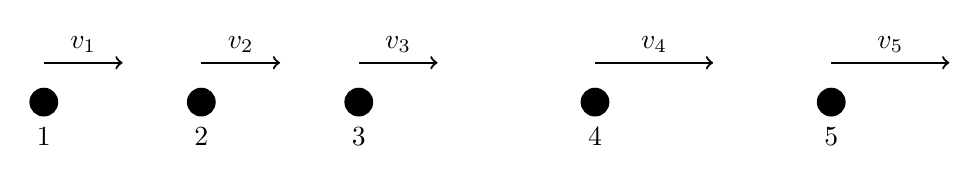
\begin{tikzpicture}
		\foreach \x in {1,2,3}
			\filldraw (2*\x,0) circle (5pt);
		\foreach \x in {1,2,3}
			\node[anchor=north] at (2*\x,-0.2) {\x};
		\foreach \x in {1,2,3}
			\draw[thick,->] (2*\x,0.5) -- (2*\x+1,0.5);
		\foreach \x in {1,2,3}
			\node[anchor=south] at (2*\x+0.5,0.5) {$v_{\x}$};
		\begin{scope}[shift={(-3,0)}]
			\foreach \x in {4,5}
				\filldraw (3*\x,0) circle (5pt);
			\foreach \x in {4,5}
				\node[anchor=north] at (3*\x,-0.2) {\x};
			\foreach \x in {4,5}
				\draw[thick,->] (3*\x,0.5) -- (3*\x+1.5,0.5);
			\foreach \x in {4,5}
				\node[anchor=south] at (3*\x+0.75,0.5) {$v_{\x}$};
		\end{scope}
	\end{tikzpicture}
\end{figure}
\end{PresentSpace}
\newpage
\begin{TeacherMargin}
\noindent\textbf{Explanations}

\noindent\textbf{L2-1: Comparing Motion Diagrams}

\noindent\textbf{Principles}
\begin{itemize}
	\item $\vec{v}_{avg} = \frac{\Delta\vec{r}}{\Delta t}$
	\item For a motion diagram, the time intervals are the same.
\end{itemize}
\noindent\textbf{Reasoning}

\noindent\textit{Method 1:}

Let us look at the beginning and end of the motion. Each object starts and ends at the same spot:
\[
\Delta\vec{r}_{1} = \Delta\vec{r}_{2} = \Delta\vec{r}.
\]
Object 2 takes more time to get to the final position:
\[
\Delta t_{2} > \Delta t_{1}.
\]
Now we have
\[
\vec{v}_{avg,1} = \frac{\Delta\vec{r}_{1}}{\Delta t_{1}}, \qquad \vec{v}_{avg,2} = \frac{\Delta\vec{r}_{2}}{\Delta t_{2}}.
\]
Since $\Delta\vec{r}$ is the same for both, a larger number in the denominator gives a smaller overall number. Therefore
\[
\left|\vec{v}_{avg,1}\right| > \left|\vec{v}_{avg,2}\right|.
\]

\noindent\textit{Method 2:}

Since the velocity appears to be constant (that is, $\Delta\vec{r}$ between two adjacent spots is the same), we can also look at individual positions.

For object 1, $\Delta\vec{r}$ between times 1 and 2 is greater than for object 2:
\[
\Delta\vec{r}_{1} > \Delta\vec{r}_{2}.
\]
The time between these two points is the same for both objects:
\[
\Delta t_{1} = \Delta t_{2} = \Delta _{t}.
\]
Now we have
\[
\vec{v}_{avg,1} = \frac{\Delta\vec{r}_{1}}{\Delta t}, \qquad \vec{v}_{avg,2} = \frac{\Delta\vec{r}_{2}}{\Delta t}.
\]
The denominators are the same, so having a larger number in the numerator gives a larger overall number. Therefore
\[
\left|\vec{v}_{avg,1}\right| > \left|\vec{v}_{avg,2}\right|.
\]

\noindent\textbf{Conclusion}

The average speed of object 1 is \underline{greater than} the average speed of object 2:
\[
\left|\vec{v}_{avg,1}\right| > \left|\vec{v}_{avg,2}\right|.
\]
\end{TeacherMargin}
\begin{PresentSpace}
\vspace{-0.5cm}
\section*{L2-1: Comparing Motion Diagrams}
\vspace{-0.2cm}
The diagrams below show the motion of two different objects. Is the average velocity of the upper object greater than, less than, or equal to the average velocity of the lower object? Explain your reasoning.
\vspace{0.3cm}
\begin{figure}[h]
	\centering
	\begin{tikzpicture}
		\node at (0.75,0) {Object 1};
		\foreach \x in {1,2,3,4,5}
			\filldraw (3*\x,0) circle (5pt);
		\foreach \x in {1,2,3,4,5}
			\node[anchor=north] at (3*\x,-0.2) {\x};
		\begin{scope}
			\node at (0.75,-1.5) {Object 2};
			\foreach \x in {1,2,3,4,5,6}
				\filldraw (2.4*\x+0.6,-1.5) circle (5pt);
			\foreach \x in {1,2,3,4,5,6}
				\node[anchor=north] at (2.4*\x+0.6,-1.7) {\x};
		\end{scope}
		\node at (7.5,-4) {\includegraphics[scale=0.4]{ExplanationsInPhysics.png}};
	\end{tikzpicture}
\end{figure}
\end{PresentSpace}
\newpage
\begin{TeacherMargin}
\noindent\textbf{L2-2 Thrown Ball}

The ball goes up, slows down, comes to a brief stop, turns around, and falls back down, increasing in speed.

\noindent\textbf{Analyze and Represent}

\noindent\textbf{1a: Understand the Problem}
\begin{itemize}
	\item $\vec{r}$: position of the ball
	\item $t$: time
	\item $\vec{v}_{i}$: initial velocity
\end{itemize}
\noindent\textbf{1b: Identify Assumptions}
\begin{itemize}
	\item The ball is thrown in a straight line.
	\begin{itemize}
		\item This simplification allows us to consider motion in only one dimension.
	\end{itemize}
	\item The ball is released and caught at the same spot.
	\begin{itemize}
		\item An actual toss and catch isn't going to be perfect, but small, random differences in starting and ending height are a minor detail that we don't need to bother with when looking at this general sort of motion.
	\end{itemize}
	\item Particle model.
	\begin{itemize}
		\item This assumption allows us to ignore any ambiguity in the object's position (we don't have to decide to measure from the center, top, or bottom), and to ignore any rotational motion the object may have about its own axis.
	\end{itemize}
\end{itemize}
\noindent\textbf{1c: Represent Physically}

\begin{figure}[h]
	\centering
	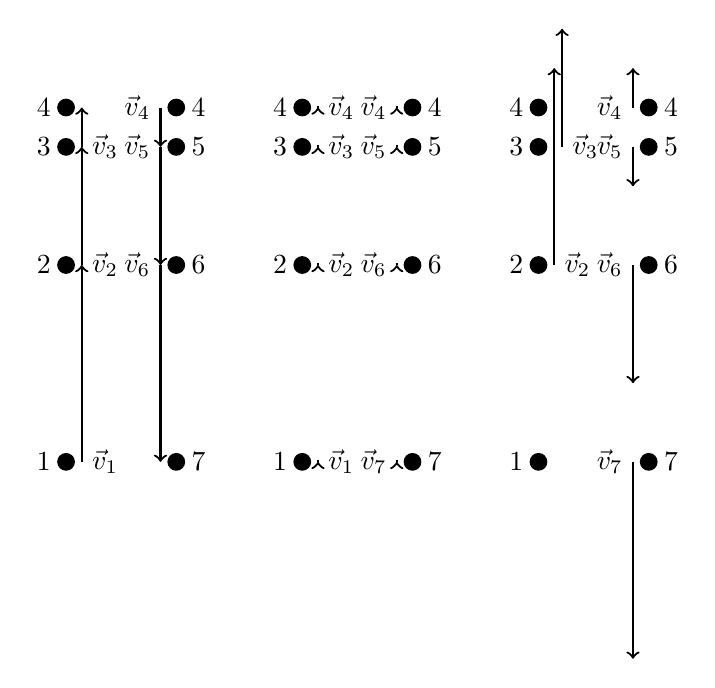
\begin{tikzpicture}
		\begin{scope}[shift={(-3.7,0)}]
			\foreach \t in {1,2,3,4}
				\filldraw (0,{-0.5*(\t-4)*(\t-4)}) circle (3pt) node[anchor=east,shift={(-2pt,0)}] {$\t$};
			\foreach \t in {1,2,3}
				\draw[thick,->] (0.2,{-0.5*(\t-4)*(\t-4)}) node[anchor=west,shift={(0,0)}] {$\vec{v}_{\t}$} -- (0.2,{-0.5*(\t-3)*(\t-3)});
		\end{scope}
		\begin{scope}[shift={(-2.3,0)}]
			\foreach \t in {4,5,6,7}
				\filldraw (0,{-0.5*(\t-4)*(\t-4)}) circle (3pt) node[anchor=west,shift={(2pt,0)}] {$\t$};
			\foreach \t in {4,5,6}
				\draw[thick,->] (-0.2,{-0.5*(\t-4)*(\t-4)}) node[anchor=east,shift={(0,0)}] {$\vec{v}_{\t}$} -- (-0.2,{-0.5*(\t-3)*(\t-3)});
		\end{scope}
		\begin{scope}[shift={(-0.7,0)}]
			\foreach \t in {1,2,3,4}
				\filldraw (0,{-0.5*(\t-4)*(\t-4)}) circle (3pt) node[anchor=east,shift={(-2pt,0)}] {$\t$};
			\foreach \t in {1,2,3,4}
				\draw[thick,->] (0.2,{-0.5*(\t-4)*(\t-4)}) node[anchor=west,shift={(0,0)}] {$\vec{v}_{\t}$} -- (0.2,{-0.5*(\t-4)*(\t-4)});
		\end{scope}
		%\node at (0,0.3) {$\vec{v}_{4}=\vec{0}$};
		\begin{scope}[shift={(0.7,0)}]
			\foreach \t in {4,5,6,7}
				\filldraw (0,{-0.5*(\t-4)*(\t-4)}) circle (3pt) node[anchor=west,shift={(2pt,0)}] {$\t$};
			\foreach \t in {4,5,6,7}
				\draw[thick,->] (-0.2,{-0.5*(\t-4)*(\t-4)}) node[anchor=east,shift={(0,0)}] {$\vec{v}_{\t}$} -- (-0.2,{-0.5*(\t-4)*(\t-4)});
		\end{scope}
		\begin{scope}[shift={(2.3,0)}]
			\foreach \t in {1,2,3,4}
				\filldraw (0,{-0.5*(\t-4)*(\t-4)}) circle (3pt) node[anchor=east,shift={(-2pt,0)}] {$\t$};
			\foreach \t in {2,3}
				\draw[thick,->] (0.1*\t,{-0.5*(\t-4)*(\t-4)}) node[anchor=west,shift={(0,0)}] {$\vec{v}_{\t}$} -- (0.1*\t,{-(\t-4)*(\t-4)+0.5*(\t-5)*(\t-5)});
		\end{scope}
		\begin{scope}[shift={(3.7,0)}]
			\foreach \t in {4,5,6,7}
				\filldraw (0,{-0.5*(\t-4)*(\t-4)}) circle (3pt) node[anchor=west,shift={(2pt,0)}] {$\t$};
			\foreach \t in {4,5,6,7}
				\draw[thick,->] (-0.2,{-0.5*(\t-4)*(\t-4)}) node[anchor=east,shift={(0,0)}] {$\vec{v}_{\t}$} -- (-0.2,{-(\t-4)*(\t-4)+0.5*(\t-5)*(\t-5)});
		\end{scope}
	\end{tikzpicture}
\end{figure}
\end{TeacherMargin}
\begin{PresentSpace}
\vspace{-0.5cm}
\section*{L2-2: Thrown Ball}
\vspace{-0.2cm}
A ball is thrown straight into the air.
\begin{itemize}
	\item Describe the motion in words (use complete sentences).
	\item Identify any quantities of interest with a symbol.
	\item Draw a motion diagram for the ball.
	\item Discuss any assumptions or idealizations you want to make.
\end{itemize}
\vspace{12cm}
\begin{figure}[h]
	\centering
	\includegraphics[scale=0.4]{AnalyzeAndRepresent.png}
\end{figure}
\end{PresentSpace}
\newpage
\begin{TeacherMargin}
\begin{figure}[h]
	\centering
	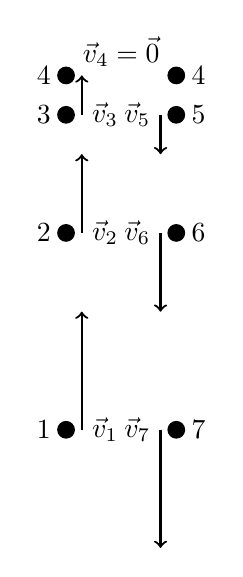
\begin{tikzpicture}
		\begin{scope}[shift={(-0.7,0)}]
			\foreach \t in {1,2,3,4}
				\filldraw (0,{-0.5*(\t-4)*(\t-4)}) circle (3pt) node[anchor=east,shift={(-2pt,0)}] {$\t$};
			\foreach \t in {1,2,3}
				\draw[thick,->] (0.2,{-0.5*(\t-4)*(\t-4)}) node[anchor=west,shift={(0,0)}] {$\vec{v}_{\t}$} -- (0.2,{-0.5*(\t-4)-0.5*(\t-4)*(\t-4)});
		\end{scope}
		\node at (0,0.3) {$\vec{v}_{4}=\vec{0}$};
		\begin{scope}[shift={(0.7,0)}]
			\foreach \t in {4,5,6,7}
				\filldraw (0,{-0.5*(\t-4)*(\t-4)}) circle (3pt) node[anchor=west,shift={(2pt,0)}] {$\t$};
			\foreach \t in {5,6,7}
				\draw[thick,->] (-0.2,{-0.5*(\t-4)*(\t-4)}) node[anchor=east,shift={(0,0)}] {$\vec{v}_{\t}$} -- (-0.2,{-0.5*(\t-4)-0.5*(\t-4)*(\t-4)});
		\end{scope}
	\end{tikzpicture}
\end{figure}
\end{TeacherMargin}
\begin{PresentSpace}

\end{PresentSpace}
\newpage
\begin{TeacherMargin}

\end{TeacherMargin}
\begin{PresentSpace}

\end{PresentSpace}
\newpage
\begin{TeacherMargin}

\end{TeacherMargin}
\begin{PresentSpace}

\end{PresentSpace}
\newpage
\begin{TeacherMargin}

\end{TeacherMargin}
\begin{PresentSpace}
\textbf{Main Ideas}
\begin{itemize}
	\item The motion of an object can be characterized by quantities like position, velocity, and acceleration.
	\item Velocity is defined as the time rate of change of position.
	\item Acceleration is defined as the time rate of change of velocity.
\end{itemize}
\end{PresentSpace}
\end{document}